% Euclidean Handout Number Thirteen
\documentclass{tufte-handout}

%\geometry{showframe}% for debugging purposes -- displays the margins

%%%% Packages to make things pretty
\usepackage{amsmath,amsthm}
\usepackage{booktabs}
\usepackage{graphicx}
\setkeys{Gin}{width=\linewidth,totalheight=\textheight,keepaspectratio}
\graphicspath{{graphics/}}
\usepackage{units}
\usepackage{fancyvrb}
\fvset{fontsize=\normalsize}
\usepackage{multicol}
\usepackage{pdfpages}

%%%% Theorem Environments
\theoremstyle{definition}
\swapnumbers
\newtheorem{problem}{Problem}[section]
\newtheorem{conjecture}[problem]{Conjecture}
\newtheorem*{definition}{Definition}
\newtheorem*{theorem}{Theorem}
\newtheorem{question}[problem]{Question}
\newtheorem{challenge}[problem]{Challenge}
\newtheorem*{postulate}{Postulate}

%%%%%

\title{Euclidean Geometry:\\An Introduction to Mathematical Work}
\author[]{Math 3600}
\date{Fall 2020}

\begin{document}

\maketitle

\begin{marginfigure}
    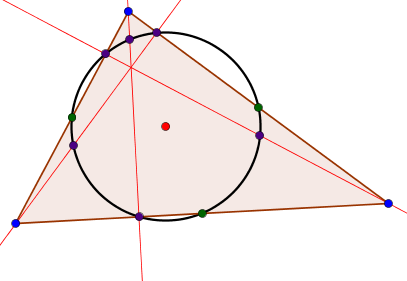
\includegraphics{NPC}
\end{marginfigure}

\setcounter{section}{13}
\section{The Theory of Content}

Read the parts of the \emph{Elements} that have to do with the basic theory of area. These are Book I, Propositions 35-48, Book II, and Book III, Propositions 35-37.

Euclid usually calls two planar figures ``equal" without explanation. 
From the work that he does, it seems that he means equality of area, or something like it, but he never defines an ``area function'' which assigns a (non-negative, real) number to each planar figure. 
Looking more closely at the text, it appears that Euclid is using a new undefined term and assuming some ``common sense" axioms to control use of the word. 
For clarity, we try to make things more explicit here.
\marginnote{This follows the basic structure of axiomatic work. We have a new undefined term, and the axioms are in place to make sure that we have concrete and specific rules for the allowable use of that new term. In this case, the axioms are basically restatements of Euclid's common notions.}
We introduce a new undefined term \emph{equal content} which satisfies the following axioms:
\begin{compactdesc}
\item[(EC1)] Congruent figures have equal content.
\item[(EC2)] If each of two figures each have equal content with a third figure, then the two figures have equal content.
\item[(EC3)] If pairs of figures with equal content are ``added," in the sense of being joined without overlap to make bigger figures, then these added figures have equal content.
\item[(EC4)] The same holds for ``subtraction,'' noting that it is immaterial where the equal figures are removed.
\item[(EC5)] Halves of figures with equal content have equal content, and doubles of figures with equal content have equal content.
\item[(EC6)] The whole is greater than the part, so if one figure is properly contained in another, then the two figures cannot have equal content.
\end{compactdesc}

\begin{center}\textit{Attention! Attention!}\end{center}

Note that Euclid never uses algebra. (It hadn't been invented, yet.) So there are no equations in his work. We shall not use them either! Writing a ``Euclid-style proof'' demands no equations. 

\clearpage

For the following tasks, work in the style of Euclid using any result from the first three books.

\begin{problem}\label{prob:present-pythagoras} 
Prepare a presentation of Euclid's beautiful proof of Proposition I.47.
\end{problem}

\begin{conjecture}\label{conj:false-area}
Let $ABC$ and $DEF$ be triangles. Let $X$ be the midpoint of $DE$, $Y$ the midpoint of $BC$. If $AB$ is congruent to $DX$ and $EF$ is congruent to $BY$, then $ABC$ and $DEF$ have equal content.
\end{conjecture}


\begin{problem}\label{prob:expand-false-area}
Expand on the statement of the last conjecture--find some theorems and prove them.
\end{problem}

\begin{problem}\label{prob:RASS-area} 
The \emph{hypotenuse-leg} Theorem 7.2 can be proved using the theory of equal content. Find such a proof.
\end{problem}

\begin{question}
There are two ways to inscribe a square in an isosceles right triangle. Which one has the greater content?
\end{question}

\begin{conjecture}[The Parallelogram Law]\label{conj:parallelogram-law}
Let $ABCD$ be a parallelogram. Then the squares on the diagonals taken together have equal content with the squares on the four sides taken together.
\end{conjecture}



\begin{problem}\label{prob:rectify-triangle}
Given a triangle $ABC$ and a segment $DE$, construct a rectangle with equal content to $ABC$ and with $DE$ as one side.
\end{problem}

\begin{problem}\label{prob:quadrature-of-rectangle}
Given a rectangle, construct a square of equal content.
\end{problem}



\vfill
\end{document}
